\thispagestyle{toancuabinone}
\pagestyle{toancuabi}
\everymath{\color{toancuabi}}
\blfootnote{$^1$\color{toancuabi}Trường Liên cấp Hội nhập Quốc tế iSchool Quảng Trị.}
\graphicspath{{../toancuabi/pic/}}
\begingroup
\AddToShipoutPicture*{\put(0,616){\includegraphics[width=19.3cm]{../bannertoancuabi}}}  
\AddToShipoutPicture*{\put(48,555){\includegraphics[scale=1]{../tieude10.pdf}}}   
\centering
\endgroup
\vspace*{152pt} 

\begin{multicols}{2}
	\textbf{\color{toancuabi}Ayatori} (hay trò chơi dây) là một trò chơi mà khi nhắc đến chắc chắn những người hâm mộ bộ truyện tranh Doraemon đều biết đến và nhớ ngay tới nhân vật Nobita. Trò chơi Ayatori là một trò chơi rất thú vị, người chơi sẽ sử dụng một sợi dây được buộc thành hình tròn, sau đó dùng những ngón tay của mình đan xen các sợi dây để tạo ra nhiều hình dạng khác nhau từ đơn giản đến phức tạp. Hôm nay, em hãy thử xếp hình ngôi sao thông qua trò chơi Ayatori nhé!
	\vskip 0.1cm
	\textit{Bước} $1$: Cách cầm dây khi mới bắt đầu chơi trò chơi Ayatori là giữ sợi dây trong ngón cái và ngón út bằng hai tay, rồi kéo ngang để chuẩn bị chơi.
	\begin{figure}[H]
		\vspace*{-10pt}
		\centering
		\captionsetup{labelformat= empty, justification=centering}
		\includegraphics[width=0.82\linewidth]{1a}
		
		\vspace*{1pt}
		\includegraphics[width=0.82\linewidth]{1b}
		
		\vspace*{1pt}
		\hspace*{1pt}\includegraphics[width=0.82\linewidth]{1c}
%		\vspace*{-10pt}
	\end{figure}
	\textit{Bước} $2$: Thả dây ở hai ngón tay út. Sau đó dùng hai ngón tay út luồn phía dưới sợi dây ở hai ngón cái để kéo sợi dây ra như hình vẽ.
	\begin{figure}[H]
		\vspace*{-5pt}
		\centering
		\captionsetup{labelformat= empty, justification=centering}
		\includegraphics[width=0.8\linewidth]{2a}

		\vspace*{1pt}
		\includegraphics[width=0.8\linewidth]{2b}
		\vspace*{-10pt}
	\end{figure}
	\textit{Bước} $3$: Lấy ngón trỏ tay phải móc vào phần dây giữa ngón cái và ngón út của tay trái. Thực hiện tương tự với ngón trỏ tay trái.
	\begin{figure}[H]
		\vspace*{-5pt}
		\centering
		\captionsetup{labelformat= empty, justification=centering}
		\includegraphics[width=0.8\linewidth]{3a}
		
		\vspace*{1pt}
		\includegraphics[width=0.8\linewidth]{3b}
%		
		\vspace*{1pt}
		\includegraphics[width=0.8\linewidth]{3c}
%		
%		\vspace*{1pt}
%		\hspace*{1pt}\includegraphics[width=1\linewidth]{3d}
%		\vspace*{-10pt}
	\end{figure}
		\begin{figure}[H]
		\vspace*{5pt}
		\centering
		\captionsetup{labelformat= empty, justification=centering}
%		\includegraphics[width=0.8\linewidth]{3a}
%		
%		\vspace*{1pt}
%		\includegraphics[width=0.8\linewidth]{3b}
%		%		
%		\vspace*{1pt}
%		\includegraphics[width=0.8\linewidth]{3c}
		\hspace*{1pt}\includegraphics[width=0.8\linewidth]{3d}
		\vspace*{-10pt}
	\end{figure}
	\textit{Bước} $4$: Thả dây ở hai ngón tay út.
	\begin{figure}[H]
		\vspace*{-5pt}
		\centering
		\captionsetup{labelformat= empty, justification=centering}
		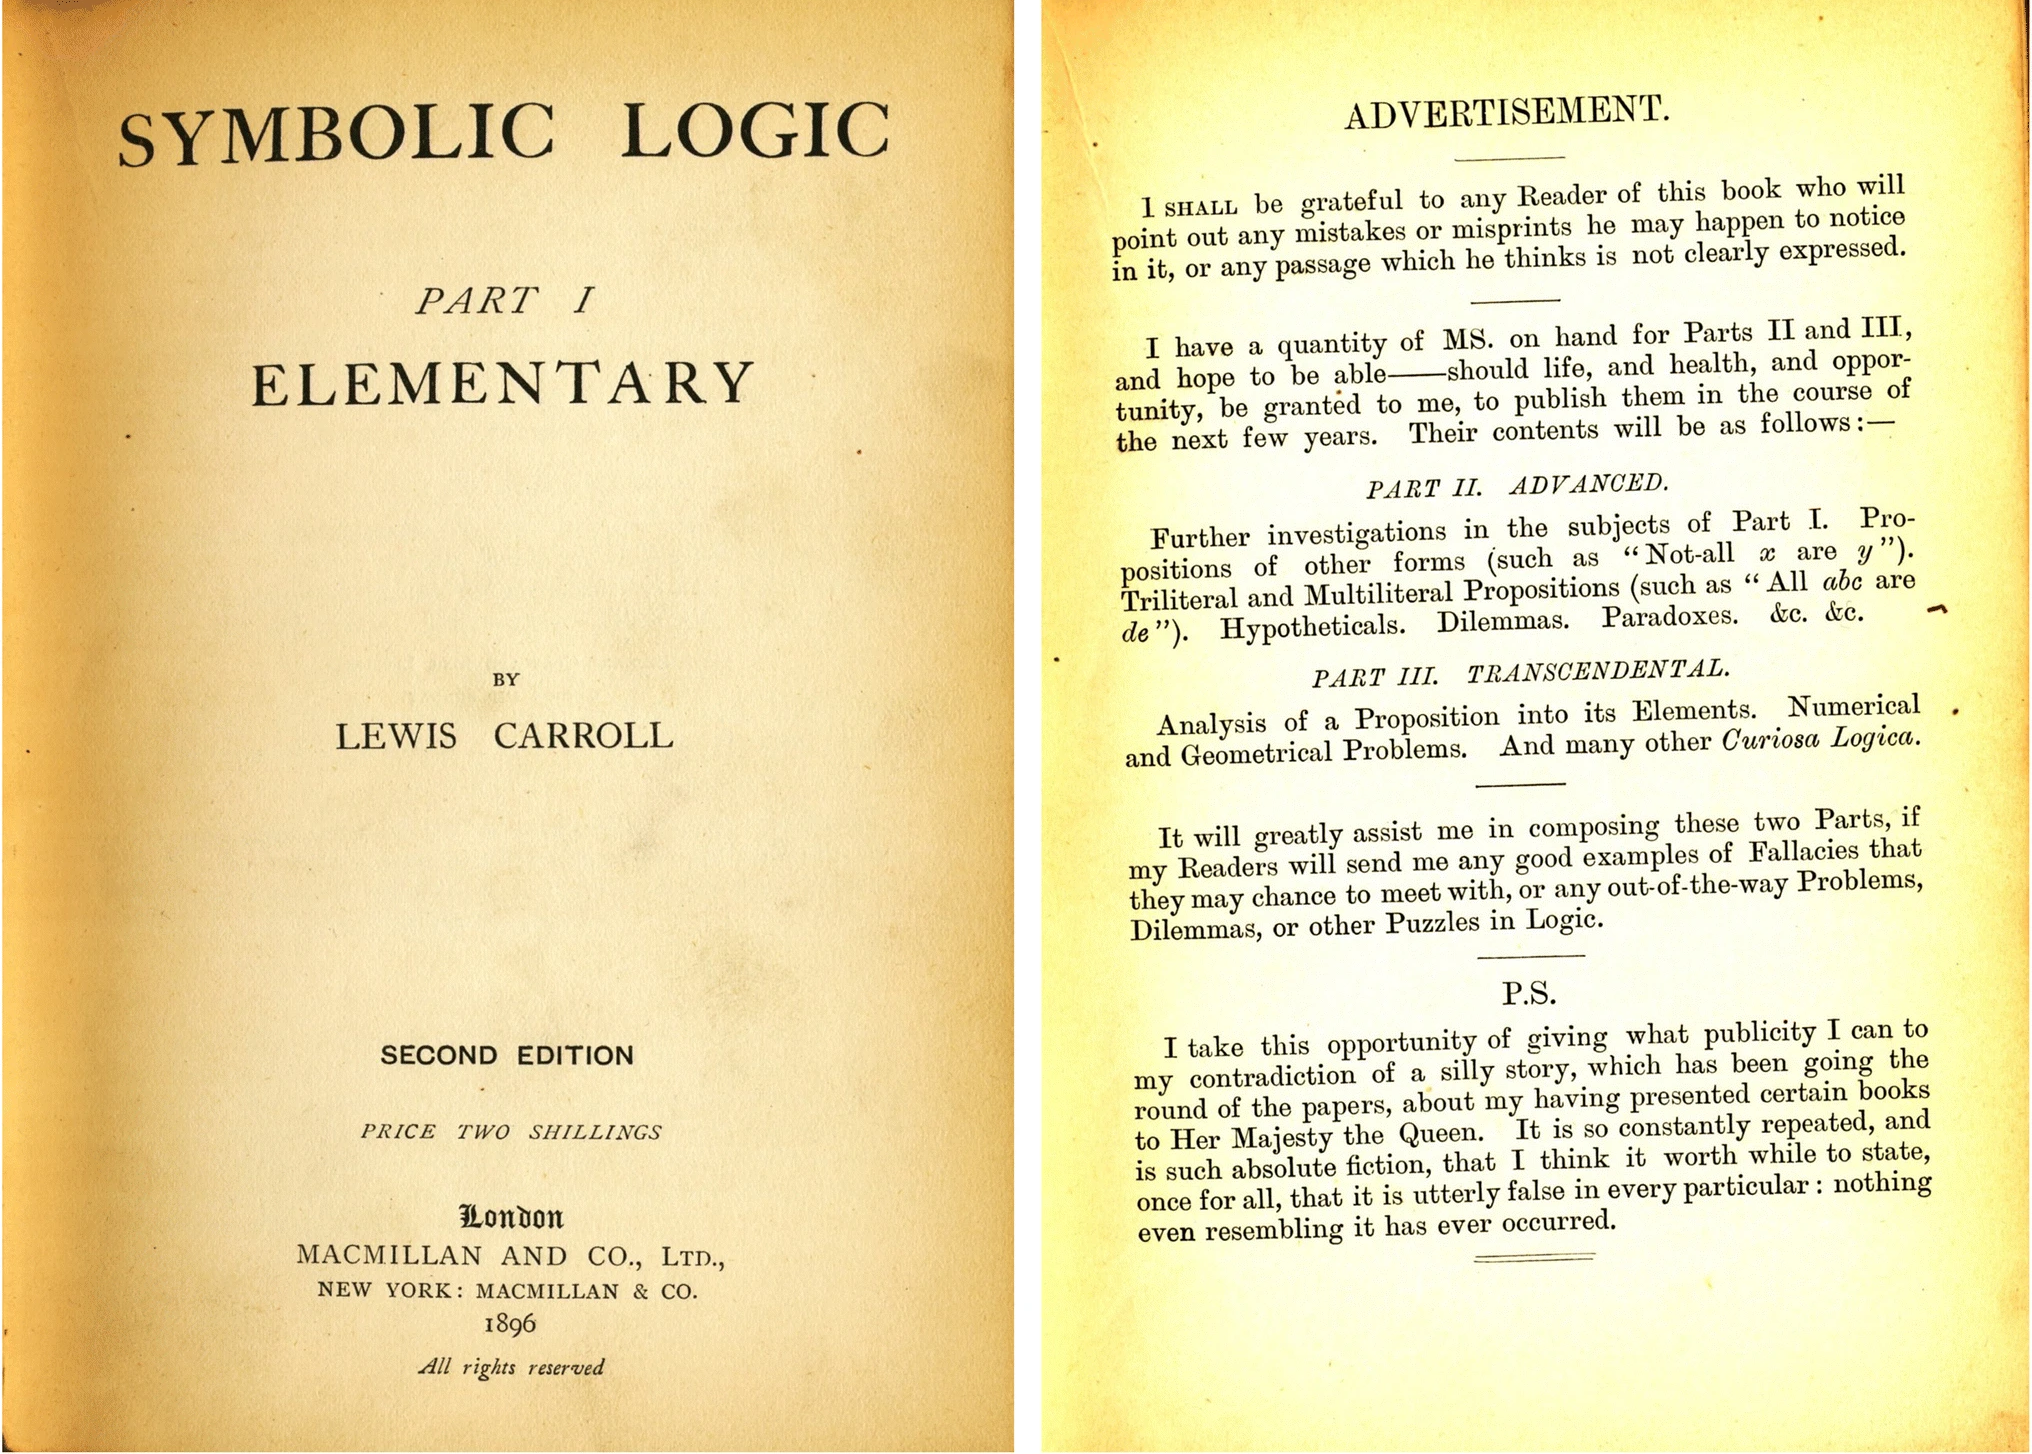
\includegraphics[width= 0.8\linewidth]{4}
%		\caption{\small\textit{\color{}}}
		\vspace*{-10pt}
	\end{figure}
	\textit{Bước} $5$: Dùng ngón út để kéo sợi dây ở dưới cùng lên và chúng ta sẽ hoàn hành ngôi sao năm cánh.
	\begin{figure}[H]
		\vspace*{5pt}
		\centering
		\captionsetup{labelformat= empty, justification=centering}
		\includegraphics[width= 0.8\linewidth]{5}
%		\caption{\small\textit{\color{}}}
		\vspace*{-5pt}
	\end{figure}
	Hãy thử suy ngẫm xem hình ngôi sao năm cánh em vừa tạo ra có bao nhiêu trục đối xứng?
	\vskip 0.1cm
	\textbf{\color{toancuabi}Làm cây thông Noel}
	\vskip 0.1cm
	\textit{Bước} $1$: Xếp hai tờ giấy màu cứng chồng lên nhau rồi gấp đôi lại cho đều nhau. Sau đó lấy bút vẽ phác họa hình cây thông lên mặt ngoài của tờ giấy rồi dùng kéo cắt theo các đường đã vẽ sẵn. Lúc mở ra, em sẽ có hai cây thông với kích thước giống nhau.
	\begin{figure}[H]
		\vspace*{-5pt}
		\centering
		\captionsetup{labelformat= empty, justification=centering}
		\includegraphics[width= 1\linewidth]{6}
%		\caption{\small\textit{\color{}}}
		\vspace*{-15pt}
	\end{figure}
	\textit{Bước} $2$: Gấp đôi cây thông theo chiều ngang, gấp đầu nhọn xuống dưới để xác định tâm của mỗi cây thông. Tiếp đến dùng kéo cắt một đường từ đỉnh cây thông xuống điểm vừa đánh dấu. Cây thông còn lại thì cắt từ đáy lên điểm vừa đánh dấu.
	\begin{figure}[H]
		\vspace*{-5pt}
		\centering
		\captionsetup{labelformat= empty, justification=centering}
		\includegraphics[width= 1\linewidth]{7}
%		\caption{\small\textit{\color{}}}
		\vspace*{-15pt}
	\end{figure}
	\textit{Bước} $3$: Sau khi đã hoàn thành việc cắt hai cây thông, em hãy ghép chúng lại với nhau theo các khe đã cắt, chú ý để các góc không bị cong. Nếu sau khi ráp cây thông bị lung lay các em có thể cố định lại bằng keo dán.
	\begin{figure}[H]
		\vspace*{-5pt}
		\centering
		\captionsetup{labelformat= empty, justification=centering}
		\includegraphics[width= 1\linewidth]{8}
%		\caption{\small\textit{\color{}}}
		\vspace*{-15pt}
	\end{figure}
	\textit{Bước} $4$: Cuối cùng các em chỉ cần điều chỉnh sao cho cây thông đứng vững, trang trí thêm các dây ruy băng hay rắc kim tuyến,... hoặc vẽ họa tiết lên cây thông Noel để nhìn đẹp hơn.
	\begin{figure}[H]
		\vspace*{-5pt}
		\centering
		\captionsetup{labelformat= empty, justification=centering}
		\includegraphics[height= 0.31\linewidth]{9a}
		\includegraphics[height= 0.31\linewidth]{9b}
		\includegraphics[height= 0.31\linewidth]{9c}
		\caption{\small\textit{\color{toancuabi}Ảnh: Internet.}}
		\vspace*{-10pt}
	\end{figure}
%	\textbf{\color{toancuabi}Bài tập}
%	\vskip 0.1cm
%	Còn gì tuyệt vời hơn khi được thả diều dưới bầu trời xanh và trong làn gió mát của những buổi chiều mùa hè oi ả. Bằng những kiến thức của bài ``Hình có trục đối xứng" và trí tưởng tượng phong phú của mình, em hãy tự làm ra cho mình một con diều đẹp đẽ với màu sắc rực rỡ nhé. Chúc em thành công!
%	\begin{figure}[H]
%		\vspace*{-5pt}
%		\centering
%		\captionsetup{labelformat= empty, justification=centering}
%		\includegraphics[width= 1\linewidth]{10}
%		\caption{\small\textit{\color{toancuabi}Hình ảnh con diều (Ảnh: Internet)}}
%		\vspace*{-10pt}
%	\end{figure}
\end{multicols}
\newpage
\begingroup
\AddToShipoutPicture*{\put(70,620){\includegraphics[scale=1]{../tieude1.pdf}}} 
\centering
\endgroup
\vspace*{85pt}

\begin{multicols}{2}
	Trong chương trình phổ thông của Việt Nam, toán tổ hợp đếm được giới thiệu ở cấp THPT. Tuy nhiên trong một số cuộc thi học sinh giỏi toán dành cho cấp tiểu học và đầu cấp PTCS thì phần tổ hợp đếm đã được đưa vào nội dung bài thi khá nhiều, ví dụ như một số cuộc thi khá phổ biến ở Việt Nam hiện nay như IMAS (International Mathematics Assessment), Apmops (The Asia Pacific Mathematical Olympiad for Primary Schools), IMSO (The International Mathematics and Science Olympiad)...
	\vskip 0.1cm
	Trong bài viết này chúng ta cùng làm quen với một số bài toán về đếm tổ hợp trong một số cuộc thi học sinh giỏi cấp tiểu học và lớp $6$ THCS.
	\vskip 0.1cm
	Trước hết chúng ta làm quen với một số khái niệm cơ bản trong phần toán tổ hợp đếm.
	\begin{figure}[H]
			\centering
			\vspace*{-5pt}
			\captionsetup{labelformat=empty, justification=centering}
			\includegraphics[width=0.9\linewidth]{_1}
			\caption{\small\textit{\color{toancuabi}Quy tắc cộng trong tam giác Pascal.}}
			\vspace*{-10pt}
		\end{figure}
	\textbf{\color{toancuabi}Quy tắc cộng, quy tắc nhân:} Quy tắc cộng và quy tắc nhân là hai quy tắc đếm cơ bản, có nội dung có thể được mô tả như sau:
	\vskip 0.1cm
	Có hai công việc gọi là Job $1$ và Job $2$ (có thể mở rộng ra nhiều hơn $2$ công việc) được thực hiện một cách độc lập nhau. Có $m$ cách thực hiện Job $1$ và $n$ cách thực hiện Job $2$, khi đó hai quy tắc đếm cơ bản được phát biểu như sau:
	\vskip 0.1cm
	\textbf{\color{toancuabi}Quy tắc cộng:} Có $m+n$ cách để thực hiện Job $1$ hoặc Job $2$.
	\vskip 0.1cm
	\textbf{\color{toancuabi}Quy tắc nhân:} Có $m\times n$ cách để thực hiện Job$1$ và Job$2$ (thực hiện cả hai công việc).
	\begin{figure}[H]
		\centering
		\vspace*{-5pt}
		\captionsetup{labelformat=empty, justification=centering}
		\includegraphics[width=1\linewidth]{_2}
		\caption{\small\textit{\color{toancuabi}Quy tắc nhân trong bài toán đếm đường đi.}}
		\vspace*{-10pt}
	\end{figure}
	\textbf{\color{toancuabi}Giai thừa:} của $n$ là số cách sắp xếp thứ tự của $n$ phần tử trong một tập hợp, được ký hiệu là $n!$ và có công thức là: $n!=1\times 2\times 3\times \ldots\times n $.
	\vskip 0.1cm
	Ghi chú: $0!=1$
	\begin{figure}[H]
		\centering
		\vspace*{-5pt}
		\captionsetup{labelformat=empty, justification=centering}
		\includegraphics[width=1\linewidth]{_3}
		\vspace*{-15pt}
	\end{figure}
	\vskip 0.1cm
	\textbf{\color{toancuabi}Hoán vị (Permutation):} Có $n$ người và chỉ có $k$ cái ghế trên một hàng ($k\le n$), ta cần xếp đủ $k$ người từ nhóm $n$ người vào $k$ cái ghế. Khi đó số cách xếp gọi là hoán vị và ký hiệu là:
	\begin{align*}
		P(n,k)&=n\!\times\!(n\!-\!1)\!\!\times\!\!(n\!-\!2)\!\!\times\!\!\ldots\!\!\times\!\!(n\!-\!k\!+\!1\!)\\
		&= \frac{n!}{(n-k)!} 
	\end{align*}
	\vskip 0.1cm
	Trong trường hợp có $n$ người và có đúng $n$ cái ghế khi đó ta có số cách sắp xếp $n$ người này chính là định nghĩa của $n!$ (số cách sắp xếp các phần tử của một tập hợp $n$ phần tử): $P(n,n)=n!$
	\begin{figure}[H]
		\centering
		\vspace*{-10pt}
		\captionsetup{labelformat=empty, justification=centering}
		\includegraphics[width=1\linewidth]{_4}
		\vspace*{-15pt}
	\end{figure}
	\vskip 0.1cm
	\resizebox{\columnwidth}{!}{{\textbf{\color{toancuabi}Hoán vị vòng tròn (Circular Permutation):}}} Xung quanh một bàn tròn có $n$ người ngồi. Hai hoán vị được coi là như nhau nếu chúng có thể chồng khít vào nhau bằng phép xuay. Số cách sắp xếp $n$ người xung quanh môt cái bàn tròn cố định là: (\textit{cố định: có nghĩa là ta không thể nhấc nó ra để lật ngược lại được})
	\begin{align*}
		P_n=(n-1)!
	\end{align*}
	Số là $(n-1)!$ thay vì $n!$ vì có $n$ cách xoay bàn và $n$ hoán vị do xoay bàn từ $1$ vị trí là như nhau.
	\begin{figure}[H]
		\centering
		\vspace*{-5pt}
		\captionsetup{labelformat=empty, justification=centering}
		\includegraphics[width=1\linewidth]{_5}
		\caption{\small\textit{\color{toancuabi}Hoán vị vòng tròn $4$ người ngồi xung quanh một cái bàn hình tròn.}}
		\vspace*{-15pt}
	\end{figure}
	\textbf{\color{toancuabi}Tổ hợp (Combonation):}  Đếm số cách để chọn $k$ người từ một nhóm $n$ người là một trong những bài toán tổ hợp đếm cơ bản, và nó được gọi bằng một cái tên đặc biệt: TỔ HỢP và được ký hiệu  $C(n,k)$; $C_n^k$ và có công thức là:
	\begin{align*}
		C_n^k&=C(n,k)=\frac{P(n,k)}{k!} \\[-0.5ex]
		&= \frac{n\!\times\!(n\!-\!1)\!\times\!(n\!-\!2)\!\times\!\ldots \!\times\!(n\!-\!k\!+\!1)}{k!}\\[-0.75ex]
		& = \frac{n!}{k!\times(n-k)!}
	\end{align*}
	\vskip 0.1cm
		\textbf{\color{toancuabi}Bài toán số $\pmb{1}$: (IMAS)}
		\vskip 0.1cm
		Sơ đồ dưới đây gồm nhiều tam giác vuông cân.
		\vskip 0.1cm
		Có bao nhiêu cách một con kiến có thể đi từ $A$ đến $C$ nếu nó chỉ được phép di chuyển lên trên, sang phải hay theo đường chéo? 
		\begin{figure}[H]
			\centering
			\vspace*{-5pt}
			\captionsetup{labelformat=empty, justification=centering}
			\includegraphics[width=0.75\linewidth]{_6}
			%	\caption{\small\textit{Hoán vị vòng tròn $4$ người ngồi xung quanh một cái bàn hình tròn.}}
			\vspace*{-15pt}
		\end{figure}
	\vskip 0.1cm
	\textbf{\color{toancuabi}Phân tích bài toán:} Tại mỗi điểm nút trên hình vẽ, số cách đi từ $A$ đến nó sẽ bằng tổng số cách đi từ $A$ đến các điểm nút ngay đằng trước nó theo chiều mũi tên được phép đi (phải, lên trên và đi chéo).
	\vskip 0.1cm
		\begin{figure}[H]
			\centering
			\vspace*{-5pt}
			\captionsetup{labelformat=empty, justification=centering}
			\includegraphics[width=0.75\linewidth]{_7}
			%	\caption{\small\textit{Hoán vị vòng tròn $4$ người ngồi xung quanh một cái bàn hình tròn.}}
			\vspace*{-15pt}
		\end{figure}
		Vậy nên ta có để điền mũi tên hướng đi và áp dụng quy tắc cộng để giải quyết các bài toán dạng này.
		\vskip 0.1cm
		\textit{Lời giải}: Theo quy tắc cộng thể hiện trên hình vẽ bên dưới ta có tổng số cách đi từ $A$ đến $C$ là $42$.
	\vskip 0.1cm
	\textbf{\color{toancuabi}Bài toán số $\pmb{2}$: (IMAS)}
	\vskip 0.1cm
	$8$ ký tự $2,0,1,5,I,M,A,S$ được xếp trên $1$ hàng. Hỏi có bao nhiêu cách xếp sao cho các chữ số đứng đằng trước các chữ cái, chữ số $0$ không đứng đầu tiên.
	\vskip 0.1cm
	\textit{Lời giải.}
	Có $8$ vị trí để xếp $8$ ký tự, các chữ số đứng đằng trước các chữ cái nên $4$ vị trí đầu tiên là các chữ số và $4$ vị trí sau cùng. Ta thực hiện $2$ công việc là xếp chữ số và xếp chữ cái:
	\vskip 0.1cm
	+ Có $3\times3\times2\times1=18$ cách xếp các chữ số (chữ số $0$ không đứng ở đầu nên vị trí đầu chỉ có $3$ cách chọn chữ số).
	\vskip 0.1cm
	+ Có $4\times3\times2\times1=4!=24$ cách xếp $4$ chữ cái.
	\vskip 0.1cm
	Theo quy tắc nhân (hai quy tắc cơ bản trong đếm tổ hợp là quy tắc cộng và quy tắc nhân) ta có số cách xếp $8$ ký tự là: $18\times24=432$.
	\vskip 0.1cm
	(Ta có thể lập luận: ta thực hiện $3$ công việc theo thứ tự là Job $1$ là viết chữ số đầu tiên, Job $2$ là viết $3$ chữ số tiếp theo, Job $3$ là viết $4$ chữ cái, và theo quy tắc nhân ta có kết quả là: $P(3,1)\times P(3,3)\times P(4,4)=3\times3!\times4!=432$)
	\vskip 0.1cm
	Mở rộng bài toán số $2$, các bạn thử sức với bài toán số $3$ nhé.
	\vskip 0.1cm
	\textbf{\color{toancuabi}Bài toán số $3$:}
	\vskip 0.1cm
	$8$ ký tự $2,0,1,5,I,M,A,S$ được xếp trên $1$ hàng. Hỏi có bao nhiêu cách xếp thỏa mãn một trong các điều kiện sau:
	\vskip 0.1cm
	$a)$ Không có hai chữ cái nào đứng cạnh nhau.
	\vskip 0.1cm
	$b)$ Chữ số $0$ nằm giữa hai chữ cái $I$ và $S$.
	\vskip 0.1cm
	$c)$ Chữ số $0$ và chữ số $1$ không đứng cạnh nhau.
	\vskip 0.1cm
	$d)$ $4$ chữ cái luôn đứng cạnh nhau.
	\vskip 0.1cm
	\textbf{\color{toancuabi}Bài toán số $4$: (IMAS)}
	\vskip 0.1cm
	Có bao nhiêu số có $3$ chữ số không chứa chữ số $3$ và chia hết cho $3$.
	\vskip 0.1cm
	\textbf{\color{toancuabi}Phân tích bài toán:}
	\vskip 0.1cm
	Gọi số có $3$ chữ số là $\overline{abc}$:
	\vskip 0.1cm
		Thử từ số nhỏ để tìm quy luật:
		\begin{align*}
			&102, 105, 108\\
			&111, 114, 117\\
			&120, 126, 129\\
			&132, 135, 138\\
			&141, 144, 147\\
			&150, 156, 159...
		\end{align*}
		Ta nhận thấy chữ số $c$ lặp theo nhóm $(2,5,8)$, $(1,4,7)$, $(0,6,9)$ và mỗi nhóm này xuất hiện phụ thuộc vào số dư chi $3$ của số $\overline{ab}$ từ đó ta có lời giải như sau:
		\vskip 0.1cm
		\textit{Lời giải}
		\vskip 0.1cm
		Nếu $\overline{ab}$ chia $3$ dư $0$ ta có $3$ cách chọn $c=\{0,6,7\}$
		\vskip 0.1cm
		Nếu $\overline{ab}$ chia $3$ dư $1$ ta có $3$ cách chọn $c=\{2,5,8\}$
		\vskip 0.1cm
		Nếu $\overline{ab}$ chia $3$ dư $2$ ta có $3$ cách chọn $c=\{1,4,7\}$
		\vskip 0.1cm
		Vậy mỗi số $\overline{ab}$ ta luôn có $3$ cách chọn chữ số $c$.
		\vskip 0.1cm
		Ta có $9\times 10$ cách tạo ra số $\overline{ab}$.
		\vskip 0.1cm
		Vậy số số có $3$ chữ số không chứa chữ số $3$ và chia hết cho $3$ là: $9\times10\times3=270$ (số);
	\vskip 0.1cm
	\textbf{\color{toancuabi}Bài toán số $5$: (APMOPS)}
	\vskip 0.1cm
	Mỗi cạnh của hình ngũ giác có cạnh $a,b,c,d,e$ tương ứng được tô bằng một trong $3$ mầu xanh, đỏ, vàng. Hỏi có bao nhiêu cách tô mầu cách cạnh của hình ngũ giác này sao cho không có $2$ cạnh nào kề nhau có cùng mầu.
		\begin{figure}[H]
			\centering
			\vspace*{-10pt}
			\captionsetup{labelformat=empty, justification=centering}
			\includegraphics[width=0.75\linewidth]{_8}
			%	\caption{\small\textit{Hoán vị vòng tròn $4$ người ngồi xung quanh một cái bàn hình tròn.}}
			\vspace*{-5pt}
		\end{figure}
		\textbf{\color{toancuabi}Phân tích bài toán:} Nếu ta tô thứ tự $a,b,c,d,e$ thì $a$ và $b$ có tương ứng $3$ và $2$ cách tô. Đến tô $c$ thông thường sẽ có $2$ cách tô, $d$ cũng $2$ cách tô, nhưng nếu như vậy thì $e$ sẽ không xác định được số cách tô vì nó phụ thuộc vào $2$ cạnh $a$ và $d$, bởi vậy ta cần xét đến mầu cụ thể của $c$ cũng như của $d$ để tính được số cách tô mầu $c$. Vậy ta có thể tiếp cận bài toán bằng hai cách sau đây.
		\vskip 0.1cm
		\textit{Lời giải $1$:}
		\vskip 0.1cm
		Tô $a$, có $3$ cách tô, tô $b$, có $2$ cách tô.
		\vskip 0.1cm
		Tô $c$:
		\vskip 0.1cm
		\textbf{\color{toancuabi}Trường hợp $1$:} $c$ cùng mầu với $a, c$ có $1$ cách tô, $d$ có $2$ cách tô, $e$ có $1$ cách tô, số cách tô ngũ giác là: $3\times2\times1\times2\times1=12$ ($1$).
		\vskip 0.1cm
		\textbf{\color{toancuabi}Trường hợp $2$:} $c$ khác mầu với $a, c$ có $1$ cách tô (vì $c$ khác với cạnh $b$ kề với nó), xét $2$ khả năng tô $d$:
		\vskip 0.1cm
		$2.1$ $d$ cùng mầu với $a, d$ có $1$ cách tô, e có $2$ cách tô. Số cách tô ngũ giác là $3\times2\times1\times2\times1=12$ ($2$).
		\vskip 0.1cm
		$2.2$ $d$ khác mầu $a, d$ có $1$ cách tô (vì $c$ khác mầu $a$), $e$ có $1$ cách tô. Số cách tô ngũ giác là: $3\times2\times1\times1\times1=6$ ($3$).
		\vskip 0.1cm
		Từ ($1$),($2$),($3$) ta có số cách tô cần tìm là: $12+12+6=30$.
	\vskip 0.1cm
	\textit{Lời giải $2$:}
	\vskip 0.1cm
	Tô $a$, có $3$ cách tô. Tô $c$, xét $2$ trường hợp:
	\vskip 0.1cm
	\textbf{\color{toancuabi}Trường hợp $1$:} $c$ cùng mầu $a, c$ có $1$ cách tô, $b$ có $2$ cách tô, $d$ có $2$ cách tô, $e$ có $1$ cách tô. Số cách tô ngũ giác là: $3\times1\times2\times2\times1=12$ ($1$).
	\vskip 0.1cm
	\textbf{\color{toancuabi}Trường hợp $2$:} $c$ khác mầu $a, c$ có $2$ cách tô, $b$ có $1$ cách tô. Xét $2$ khả năng tô $d$.
	\vskip 0.1cm
	$2.1$ $d$ cùng mầu với $a, d$ có $1$ cách tô, $e$ có $2$ cách tô. Số cách tô ngũ giác là: $3\times2\times1\times1\times2=12$ ($2$).
	\vskip 0.1cm
	$2.2$ $d$ khác mầu $a$, $d$ có $1$ cách tô (do $c$ khác mầu $a$), $e$ có $1$ cách tô. Số cách tô ngũ giác là: $3\times2\times1\times1\times1=6$ ($3$).
	\vskip 0.1cm
	Từ ($1$),($2$),($3$) ta có số cách tô cần tìm là: $12+12+6=30$.
	\vskip 0.1cm
		\textbf{\color{toancuabi}Bài toán số $6$: (Apmops)}
		\vskip 0.1cm
		$A,B,C,D,E$ và $F$ là các điểm nằm trên $2$ đường thẳng như hình vẽ. Có bao nhiêu tam giác được tạo bởi $3$ trong $6$ điểm đã cho.
		\begin{figure}[H]
			\centering
			\vspace*{-5pt}
			\captionsetup{labelformat=empty, justification=centering}
			\includegraphics[width=0.75\linewidth]{_9}
			%	\caption{\small\textit{Hoán vị vòng tròn $4$ người ngồi xung quanh một cái bàn hình tròn.}}
			\vspace*{-15pt}
		\end{figure}
	\vskip 0.1cm
	\textbf{\color{toancuabi}Phân tích bài toán:}
	\vskip 0.1cm
	Trên mặt phẳng cứ $3$ điểm phân biệt không thẳng hàng luôn tạo ra một tam giác, còn $3$ điểm phân biệt thẳng hàng thì không tạo ra một tam giác thông thưởng mà thường được gọi là tam giác suy biến (degenerate triangle). Tương tự như thế, nếu có các đường thẳng đôi một cắt nhau, mà không có $3$ đường thẳng nào cắt nhau tại $1$ điểm ($3$ đường đồng quy) thì cứ $3$ đường thẳng tạo ra được $1$ đoạn thẳng. Cứ $3$ đường thẳng đồng quy thì nó tạo ra một tam giác suy biến (có $3$ đỉnh trùng vào nhau). Các tính chất này có thể được áp dụng để giải bài toán trên và các bài toán mở rộng ở phần dưới.
	\vskip 0.1cm
	\textit{Lời giải $1$:}
	\vskip 0.1cm
	Xét $2$ trường hợp, trường hợp $1$: tam giác có đáy nằm ở đường thẳng phía dưới, đỉnh nằm ở đường thẳng phía trên, có $C(3,2)$ cách chọn đáy và $C(3,1)$ cách chọn đỉnh, theo quy tắc nhân, số tam giác đếm được là: $C(3,2)\times C(3,1)$. Tương tự, trường hợp $2$: tam giác có đáy nằm ở đường thẳng phía trên, đỉnh nằm ở đường thẳng phía dưới, có $C(3,2)$ cách chọn đáy và $C(3,1)$ cách chọn đỉnh, theo quy tắc nhân, số tam giác đếm được là: $C(3,2)\times C(3,1)$.
	\vskip 0.1cm
	Vậy số tam giác cần tìm là: $2\times C(3,2)\times C(3,1) = 2\times3\times3=18$.
	\vskip 0.1cm
	\textit{Lời giải $2$:}
	\vskip 0.1cm
	Số cách chọn ra $3$ điểm là: $C(6,3)=6\times 5\times4/3!=20$
	\vskip 0.1cm
	Số tam giác suy biến là: $3\times C(3,3)=2$
	\vskip 0.1cm
	Vậy số tam giác là: $20-2=18$
	\vskip 0.1cm
	Mở rộng bài toán số $5$, các bạn thử sức của mình xem sao nhé.
	\vskip 0.1cm
		\textbf{\color{toancuabi}Bài toán $6.1$ (Apmops)}
		\vskip 0.1cm
		Cho các điểm $A1$, $A2$, $A3$, $B1$, $B2$, $B3$, $B4$, $C1$, $C2$, $C3$, $C4$ và $C5$ nằm trên $3$ đường thẳng như hình vẽ. Có bao nhiêu tam giác được tạo bởi $3$ trong các đỉnh đã cho?
		\begin{figure}[H]
			\centering
			\vspace*{-5pt}
			\captionsetup{labelformat=empty, justification=centering}
			\includegraphics[width=0.75\linewidth]{_10}
			%	\caption{\small\textit{Hoán vị vòng tròn $4$ người ngồi xung quanh một cái bàn hình tròn.}}
			\vspace*{-15pt}
		\end{figure}
		{Bài toán $6.2$}
		Có bao nhiêu tam giác trong hình vẽ?
		\begin{figure}[H]
			\centering
			\vspace*{-10pt}
			\captionsetup{labelformat=empty, justification=centering}
			\includegraphics[width=0.75\linewidth]{_11}
			%	\caption{\small\textit{Hoán vị vòng tròn $4$ người ngồi xung quanh một cái bàn hình tròn.}}
			\vspace*{-5pt}
		\end{figure}
		{Bài toán $6.3$}
		Có bao nhiêu tam giác được tạo bởi 3 trong 12 điểm đã cho trên lưới ô vuông như hình vẽ?
		\begin{figure}[H]
			\centering
			\vspace*{-5pt}
			\captionsetup{labelformat=empty, justification=centering}
			\includegraphics[width=0.75\linewidth]{_12}
			%	\caption{\small\textit{Hoán vị vòng tròn $4$ người ngồi xung quanh một cái bàn hình tròn.}}
			\vspace*{-5pt}
		\end{figure}
	\textbf{\color{toancuabi}Bài toán số $7$: (Apmops)}
	\vskip 0.1cm
	Có bao nhiêu cách để tô $6$ mặt của một hình lập phương bằng $6$ mầu, mỗi mặt được tô bằng $1$ mầu sao cho không có hai mặt nào có cùng mầu? (Hai cách tô mầu được coi là như nhau nếu chúng nhìn giống hệt nhau sau một phép xoay hình). 
	\vskip 0.1cm
	\textbf{\color{toancuabi}Phân tích bài toán:} Hướng đi thứ nhất, ta hình dung nếu cố định hình lập phương lại và mỗi cách nhìn khác nhau ở mỗi phía được coi là khác nhau, như thế thì số cách tô sẽ như tô theo hàng ngang ($6$ người ngồi trên $6$ cái ghế trên $1$ hàng) và sẽ là $6!=720$ cách. Do hình lập phương này xoay được nên ta xem mỗi một kiểu tô có bao nhiêu cách xoay nó xung quanh chính nó. Do có $6$ mầu ta có $6$ cách xuay để có đáy khác mầu. Mỗi cách đặt đáy với $1$ mầu ta có $4$ cách xoay xung quanh chính nó (do hình lập phương có $4$ cạnh bên), từ đó ta có hướng giải quyết bài toán.
	\vskip 0.1cm
	Hướng đi thứ $2$, do hình lập phương xoay được nên ta có thể cố định mầu ở những vị trí ta có thể xuay nó về và ta sẽ có hướng giải quyết bài toán như lời giải $2$.
	\vskip 0.1cm
	Hướng đi thứ $3$ gần giống với hướng thứ $2$, ta có thể hình dung mình có thể tô mầu ở đáy bằng mầu tùy thích do hình lập phương xoay được, mặt đối diện trên đỉnh sẽ còn $5$ cách tô, $4$ mặt xung quanh ta sẽ hình dung nó như $4$ người ngồi xung quanh một cái bàn tròn nên ta có thể áp dụng bài toán hoán vị vòng tròn để giải quyết.
	\vskip 0.1cm
	\textit{Lời giải $1$:}
	\vskip 0.1cm 
	Giả sử hình lập phương cố định, khi đó ta có $6!=720$ cách tô.
	\vskip 0.1cm
	Mỗi cách tô ta có $6$ cách đặt các mặt khác mầu nhau xuống đáy, khi đặt rồi ta có $4$ cách xoay xung quanh nó, vậy ứng với mỗi cách tô mầu ta có $6\times4=24$ cách xoay nó xung quanh chính nó. Vậy số cách tô mầu là: $720:24=30$ (cách).
	\vskip 0.1cm
	\textit{Lời giải $2$:}
	\vskip 0.1cm 
	Đầu tiên ta tô mầu $1$ mặt (mầu ta thích), rồi đặt nó xuống đáy, khi đó ở mặt đối diện trên đỉnh có $5$ cách tô.
	\vskip 0.1cm
	Tiếp theo ta tô mầu $1$ mặt xung quanh (mầu ta thích trong $4$ mầu còn lại), rồi xoay nó sang bên trái, khi đó mặt bên phải có $3$ cách tô, còn $2$ mặt còn lại (trước và sau) có $2!$ cách tô, vậy số cách tô mầu là: $1\times5\times1\times3\times2!=30$ (cách)
	\vskip 0.1cm
	\textit{Lời giải $3$:}
	\vskip 0.1cm
	Tương tự như lời giải $2$, đầu tiên ta tô mầu $1$ mặt (mầu ta thích), rồi đặt nó xuống đáy, khi đó ở mặt đối diện trên đỉnh có $5$ cách tô.
	\vskip 0.1cm
	Còn $4$ mặt xung quanh, do xoay được nên theo bài toán hoán vị vòng tròn ta có $4!/4=6$ cách tô.
	\vskip 0.1cm
	Vậy số cách tô mầu hình lập phương là: $5\times 6=30$ (cách).
	\vskip 0.1cm
	\textbf{\color{toancuabi}Bài toán số $8$: (IMSO)}
	\vskip 0.1cm
	Một hình lập phương được tô các mặt bằng $6$ mầu, mỗi mặt $1$ mầu khác nhau và được đánh số từ $1$ đến $6$ sao cho tổng hai mặt đối diện bằng $7$. Hỏi có bao nhiêu cách tô mầu và đánh số hình lập phương này? (Hai cách tô mầu, đánh số được coi là như nhau nếu chúng nhìn giống hệt nhau sau một phép xoay hình). 
	\vskip 0.1cm
	Phân tích bài toán: Bài toán này là tương đối khó khi các bạn lớp $5,6$ đi thi gặp phải, và đúng là trong năm thi đó đoàn học sinh Việt Nam chỉ có đúng $1$ bạn làm được, tuy nhiên nếu chia bài toán làm hai bước, bước $1$ tô mầu, bước $2$ điền số thì ta có thể giải quyết được bài toán một cách tương đối dễ dàng.
	\vskip 0.1cm
	\textit{Lời giải:}
	\vskip 0.1cm 
	Bước $1$: Tô mầu hình lập phương, theo bài toán số $7$, ta có $30$ cách tô mầu hình lập phương này.
	\vskip 0.1cm
	Bước $2$: Đánh số, ta đánh theo thứ tự:
	\vskip 0.1cm
	Đánh số $1$, có $6$ cách. Đánh số $6$ ở mặt đối diện số $1$, có $1$ cách.
	\vskip 0.1cm
	Đánh số $2$, có $4$ cách (do còn $4$ mặt chưa đánh số). Đánh số $5$ ở mặt đối diện, có $1$ cách.
	\vskip 0.1cm
	Đánh số $3$, có $2$ cách (do còn $2$ mặt chưa đánh số). Đánh số $4$ ở mặt đối diện, có $1$ cách.
	\vskip 0.1cm
	Vậy ta có $6\times1\times4\times1\times2\times1=48$ cách đánh số.
	\vskip 0.1cm
	Theo quy tắc nhân ta có số cách tô mầu và đánh số là: $30\times 48=1440$ (cách).
	\vskip 0.1cm
	\textbf{\color{toancuabi}Bài toán số $9$: (IMAS)}
	\vskip 0.1cm
		Một bàn cờ hình vuông $5\times 5$ được xếp một hình chữ L chiếm $4$ ô như hình vẽ. Ta có thể xuay hoặc lật hình chữ L này. Hỏi có bao nhiêu cách xếp hình chữ L này vào bàn cờ hình vuông đã cho?
		\begin{figure}[H]
			\centering
			\vspace*{-10pt}
			\captionsetup{labelformat=empty, justification=centering}
			\includegraphics[width=0.4\linewidth]{_13}
			\vspace*{-15pt}
		\end{figure}
	Phân tích bài toán: Ta nhận thấy hình chữ L tô đen có thể xoay hoặc lật được, nên ta sẽ xem nó có thể có bao nhiêu cách biến hình (xoay hoặc lật).  Ứng với mỗi phép biến hình bằng xoay, lật ta xem có bao nhiêu cách trượt nó theo hàng ngang và hàng dọc, từ đó ta có cách giải quyết bài toán.
	\vskip 0.1cm
	\textit{Lời giải:}
	\vskip 0.1cm
	Ta tính số cách xoay, lật hình chữ L tô đậm, như hình dưới ta có $8$ cách.
	\begin{figure}[H]
		\centering
		\vspace*{-10pt}
		\captionsetup{labelformat=empty, justification=centering}
		\includegraphics[width=1\linewidth]{_14}
		\vspace*{-15pt}
	\end{figure}
	Ứng với mỗi cách biến hình này, ta xem có bao nhiêu cách dời hình theo hàng ngang và hàng dọc, và ta tính được số cách dời hình bằng trượt (tịnh tiến) theo hai chiều ngang, dọc là: $3\times4=12$.
	\vskip 0.1cm
		\begin{figure}[H]
			\centering
			\vspace*{-10pt}
			\captionsetup{labelformat=empty, justification=centering}
			\includegraphics[width=1\linewidth]{_15}
			\vspace*{-15pt}
		\end{figure}
		Theo quy tắc nhân, ta có số cách đặt chữ L vào ô vuông $5\times 5$ là: $8\times12=96$ (cách)
	\vskip 0.1cm
	Mở rộng bài toán số $9$. Các bạn thử sức mình xem nhé.
	\vskip 0.1cm
	Bài toán số $9.1$: Đề bài giống như bài toán số $9$, hình được xếp vào được thay đổi như sau:
	\begin{figure}[H]
		\centering
		\vspace*{-5pt}
		\captionsetup{labelformat=empty, justification=centering}
		\includegraphics[height=0.4\linewidth]{_16}\quad
		\includegraphics[height=0.4\linewidth]{_17}
		\caption{\small\textit{$a)$ \hspace*{100pt} $b)$}}
		\vspace*{-15pt}
	\end{figure}
	\textbf{\color{toancuabi}Bài toán số $10$: (IMSO).}
	\vskip 0.1cm
	Một hình tròn và một tam giác được xếp trên các điểm cắt của lưới ô vuông như hình vẽ sao cho tam giác và hình tròn không cùng nằm trên một hàng hay một cột.
	\vskip 0.1cm
		Hỏi có bao nhiêu cách xếp tam giác và hình tròn vào lưới ô vuông như hình vẽ này. Trên hình vẽ là một ví dụ về cách xếp tam giác và hình tròn.
		\begin{figure}[H]
			\centering
			\vspace*{-10pt}
			\captionsetup{labelformat=empty, justification=centering}
			\includegraphics[width=0.4\linewidth]{_18}
			\vspace*{-15pt}
		\end{figure}
	\vskip 0.1cm
	\textbf{\color{toancuabi}Phân tích bài toán:} Bài toán này các bạn nhỏ lớp $4,5$ trong câu lạc bộ toán UMC đã làm được theo nhiều cách khác nhau, các bạn quan sát sẽ thấy ngoài hai điểm ở hàng trên cùng thi bên dưới cứ mỗi hình chữ nhật sẽ có $2!\times 2!=4$ cách đặt hình tròn và tam giác (do mỗi cặp đỉnh không kề nhau của $1$ hình chữ nhật sẽ có $2!$ cách đặt hình tròn và tam giác). Sau đây là một số cách giải của các bạn.
	\vskip 0.1cm
	\textit{Lời giải $1$: }(Lê Kỳ Nam, Vĩnh Giang)
	\vskip 0.1cm
	Nếu đường tròn nằm trên hàng đầu tiên (có $2$ vị trí), thì ở mỗi vị trí sẽ có $14 - 4 - 1 = 9$ cách chọn tam giác, tổng số cách chọn là: $9 \times 2 = 18$.
	\vskip 0.1cm
	Nếu đường tròn đi vào phần còn lại của $2$ cột đầu tiên, thì ở mỗi vị trí, số cách chọn tam giác là $14 - 3 - 3 - 1 = 7$, tổng số cách chọn là $6 \times 7 = 42$.
	\vskip 0.1cm
	Nếu đường tròn đi ở $2$ cột cuối cùng, thì ở mỗi vị trí, tam giác sẽ có $14 - 3 - 2 - 1 = 8$ lựa chọn, tổng số cách chọn là $6 \times 8 = 48$.
	\vskip 0.1cm
	Tổng số cách xếp hình tròn và hình tam giác là: $18 + 42 + 48 = 108$.
	\vskip 0.1cm
	Đáp số: $108$
	\vskip 0.1cm
	\textit{Lời giải $2$:} (Nguyễn Gia Tuấn)
	\vskip 0.1cm
	Nếu hình tròn và hình tam giác không được đặt trên hình vuông trên cùng thì có $3 \times 4 \times 2 \times 3 = 72$ cách chọn.
	\vskip 0.1cm
	Nếu một trong các tam giác hoặc hình tròn được đặt trên hình vuông trên cùng thì có $2 \times 3 \times 3 \times 2 = 36$ cách chọn.
	\vskip 0.1cm
	Tổng cộng có $72 + 36 = 108$ cách chọn.
	\vskip 0.1cm
	\textit{Lời giải $3$:} (Nguyễn Trọng Cường).
	\vskip 0.1cm
	Tổng số các cách có thể đặt hình tròn và tam giác vào $2$ điểm bất kỳ của hình là: $14\times13 = 182$ cách
	\vskip 0.1cm
	Nếu hình tròn và tam giác nằm trên cùng $1$ cột, hoặc $1$ hàng, thì $2$ điểm sẽ tạo nên $1$ đoạn thẳng. Ta đếm số đoạn thẳng của hình trên.
	\vskip 0.1cm
	Số đoạn thẳng của hình là :
	\begin{align*}
		&1 + (1+2+3) \times 3 + (1+2+3) \times 2 \\
		&+ (1+2) \times 2 = 37
	\end{align*}
	Hình tròn và tam giác ở $2$ đầu đoạn thẳng, đổi chỗ được cho nhau $\Rightarrow$ có $37 \times 2 = 74$ cách ko thỏa mãn
	\vskip 0.1cm
	Số cách thỏa mãn đề bài là $182 - 74 = 108$ cách.
	\vskip 0.1cm
	\textit{Lời giải $4$:} (Nguyễn Gia Tuấn). -- Dùng phần bù:
	\vskip 0.1cm
	Với lưới ô vuông $3 \times 3$ thì ta có $C(4,2)\times C(4,2)\times 4 = 144$ cách chọn. (Do mỗi hình chữ nhật có $4$ cách đặt tam giác và hình tròn).
	\vskip 0.1cm
	Trong lưới $3 \times 3$ đó, nếu đặt hình tròn hoặc tam giác vào $2$ điểm trên cùng ở bên phải thì có $2 \times 3 \times  3 \times 2 = 36$ cách chọn.
	\vskip 0.1cm
	Vậy ta có $144 - 36 = 108$ cách chọn để xếp hình tròn và hình tam giác.
	\vskip 0.1cm
	Trả lời: $108$ lựa chọn.
\end{multicols}
\newpage
\begingroup
\AddToShipoutPicture*{\put(122,675){\includegraphics[scale=1]{../tieude.pdf}}}  
\centering
\endgroup
\vspace*{25pt} 
\begin{multicols}{2}
	Cùng với cảnh sát thành phố, thám tử Xuân Phong đã tóm gọn được một băng cướp gồm $50$ tên. Tuy nhiên khi tra hỏi, tên cướp nào cũng muốn làm giảm nhẹ tội lỗi của mình. Qua điều tra, Xuân Phong biết rằng tất cả $50$ tên chưa từng cùng tham gia một vụ cướp, tuy nhiên cứ hai tên bất kỳ trong số chúng đều đã gặp gỡ nhau tại các vụ cướp bóc chung duy nhất đúng một lần. Khi khai nhận, tất cả các tên cướp đều trả lời rằng, chúng chỉ mới đi trộm cắp cướp giật và số vụ cướp mà mỗi tên tham gia đều ít hơn $8$ vụ. Xuân Phong nghe lời khai của chúng đã xác định được ngay có ít nhất một tên cướp đã nói dối. Em có biết vì sao Xuân Phong lại kết luận được như vậy hay không?
	%	Giả sử tất cả các tên cướp đều khai thật. Ta chọn một tên cướp bất kỳ, gọi tên là $A$. Tên này tham gia không quá $7$ vụ cướp, hơn nữa $49$ tên còn lại đều chỉ tham gia đúng duy nhất một vụ cướp chung với $A$. Theo nguyên lý Dirichlet, phải có một vụ cướp (đặt tên là $T$) mà có không ít hơn $7$ tên trong số $49$ tên còn lại tham gia. Cùng với $A$, sẽ có không ít hơn $8$ tên cướp tham gia vụ cướp $T$ này. Vì $50$ tên cướp không cùng tham gia một vụ, nên phải có một tên không tham gia vụ $T$. Ta gọi đó là tên cướp $B$. 
	%	\vskip 0.1cm
	%	Ta sẽ chỉ ra $B$ tham gia ít nhất $8$ vụ cướp. Thật vậy, theo kết luận điều tra $B$ có tham gia các vụ cướp cùng với mỗi tên trong số tất cả các tên tham gia vụ $T$, hơn nữa tất cả các vụ cướp đó là khác nhau.  Nếu không, sẽ có hai vụ cướp trùng nhau. Điều đó có nghĩa là có hai tên cướp (đặt tên là $X$ và $Y$) sao cho $B,X,Y$ cùng tham gia một vụ $S$ ($S$ khác với $T$); hơn nữa $X,Y$ cũng đã tham gia cả vụ cướp $T$. Suy ra $X,Y$ cùng tham gia cả $2$ vụ cướp khác nhau là $S$ và $T$. Điều này mâu thuẫn với kết luận điều tra.
	%	\vskip 0.1cm
	%	Mâu thuẫn trên chỉ ra phải có một tên cướp khai gian dối. Điều này có nghĩa ít nhất có một tên đã tham gia không ít hơn $8$ vụ cướp.
\end{multicols}
\begin{figure}[H]
	\centering
	\vspace*{-15pt}
	\captionsetup{labelformat= empty, justification=centering}
	\includegraphics[width=0.85\linewidth]{xp}
	\vspace*{-10pt}
\end{figure}
\vspace*{-10pt}
{\color{toancuabi}\rule{1\linewidth}{0.1pt}}
\begingroup
\AddToShipoutPicture*{\put(115,315){\includegraphics[scale=1]{../tieude11.pdf}}} 
\centering
\endgroup
\vspace*{45pt}

\begin{multicols}{2}
	$\pmb{1.}$ Ở nhà một mình, bé Hoa rót ra một cốc sữa đầy và uống hết một nửa. Sau đó Hoa rót thêm nước ép táo vào cho đầy cốc, rồi lại uống hết một nửa. Cuối cùng, bé lại rót thêm nước ép táo vào đầy cốc rồi uống hết sạch cả cốc. Hỏi bé Hoa đã uống thứ gì nhiều hơn: sữa hay nước ép táo?
	\begin{figure}[H]
		\centering
		\vspace*{-5pt}
		\captionsetup{labelformat= empty, justification=centering}
		\includegraphics[width=0.9\linewidth]{Pi6_bai1}
		\vspace*{-5pt}
	\end{figure}
	$\pmb{2.}$ Dê con và Sói cùng thi xem ai chạy từ nhà tới bờ suối và quay ngược lại nhanh hơn. Biết rằng khoảng cách từ nhà tới bờ suối là $100$ bước nhảy của Dê con. Một bước nhảy của Sói dài gấp $3$ lần một bước nhảy của Dê con. Tuy nhiên trong khoảng thời gian Sói nhảy được một bước thì Dê con lại nhảy được $3$ bước. Hỏi ai sẽ chiến thắng?
	\begin{figure}[H]
		\centering
		\vspace*{-5pt}
		\captionsetup{labelformat= empty, justification=centering}
		\includegraphics[width=0.95\linewidth]{Pi6_bai2}
		\vspace*{-5pt}
	\end{figure}
	$\pmb{3.}$ 	Có tất cả $25$ chú chim cúc cu và gà trống cùng tham gia một cuộc thi hùng biện giữa các loài vật. Trong số $15$ chú chim bất kỳ luôn có ít nhất một chú gà trống, và trong số $12$ chú chim bất kỳ luôn có ít nhất một chú chim cúc cu. Hỏi trong cuộc thi đó có bao nhiêu chú gà trống và bao nhiêu chú chim cúc cu tham gia?
	\begin{figure}[H]
		\centering
		\vspace*{-5pt}
		\captionsetup{labelformat= empty, justification=centering}
		\includegraphics[width=1\linewidth]{Pi6_bai3}
		\vspace*{-10pt}
	\end{figure}
	$\pmb{4.}$ Người ta trồng trong công viên hai loài cây gồm phượng vĩ và sấu. Trong đó phượng vĩ chiếm $60\%$ tổng số hai loài. Vào mùa xuân cây sấu được trồng thêm trong công viên, do đó cây phượng vĩ chỉ còn chiếm $20\%$ tổng số cây. Sang mùa thu người ta lại trồng thêm  phượng vĩ, vì thế cây phượng vĩ lại chiếm $60\%$ tổng số cây hai loài. Hỏi sau hai lần trồng thì số cây trong công viên tăng lên bao nhiêu lần?
	\begin{figure}[H]
		\centering
		\vspace*{-5pt}
		\captionsetup{labelformat= empty, justification=centering}
		\includegraphics[width=1\linewidth]{Pi6_bai4}
		\vspace*{-10pt}
	\end{figure}
	$\pmb{5.}$ Alibaba đột nhập vào một hang động, trong đó có $100$ chiếc bao vải đựng đầy những đồng tiền. Một chiếc bao vải trong số đó chỉ đựng toàn đồng tiền giả. Khối lượng của một đồng tiền thật là $10$ gram, trong khi khối lượng của một đồng tiền giả là $9$ gram. Hỏi Alibaba làm thế nào để chỉ cân một lần duy nhất (bằng một cái cân chính xác có hiển thị số) tìm ra được bao vải chứa các đồng tiền giả?
	\begin{figure}[H]
		\centering
		\vspace*{-5pt}
		\captionsetup{labelformat= empty, justification=centering}
		\includegraphics[width=1\linewidth]{Pi6_bai5}
		\vspace*{-10pt}
	\end{figure}
	$\pmb{6.}$ 	Trên một bàn cờ $8\times8$ người ta xếp một số lớn nhất có thể các quân Tượng sao cho không có hai quân Tượng nào ``ăn" lẫn nhau. Em hãy chứng minh rằng số các cách xếp khác nhau như vậy là một số chính phương (tức là bình phương của một số tự nhiên).
	\begin{figure}[H]
		\centering
		\vspace*{-5pt}
		\captionsetup{labelformat= empty, justification=centering}
		\includegraphics[width=1\linewidth]{Pi6_bai6}
		\vspace*{-5pt}
	\end{figure}
\end{multicols}
%\newpage
%\begingroup
%\AddToShipoutPicture*{\put(110,645){\includegraphics[scale=1]{../tieude2.pdf}}} 
%\centering
%\endgroup
%\vspace*{55pt}
%
%\begin{multicols}{2}
%	$\pmb{1.}$ Một bác nông dân chở một xe ô tô quất cảnh ra chợ Tết để bán. Sau khi bán hết cây quất cuối cùng với giá $230$ nghìn đồng, bác tính nhẩm lại thấy mình đã bán số cây quất với giá trung bình là $245$ nghìn đồng/cây. Nhưng ngay lúc ấy người mua cây quất cuối quay trở lại và chỉ cho bác thấy cành quất bị rụng quá nhiều lá, nên ông ta chỉ đồng ý mua với giá $158$ nghìn đồng. 
%	Bác chấp thuận và bán cây quất đó. Khi nhẩm tính lại, bác nông dân thấy giá trung bình của xe quất bây giờ là $242$ nghìn đồng/cây. Hỏi bác đã bán được bao nhiêu cây quất?
%	\begin{figure}[H]
%		\centering
%		\vspace*{-10pt}
%		\captionsetup{labelformat= empty, justification=centering}
%		\includegraphics[width=0.7\linewidth]{Pi1_2_Bai1}
%		\vspace*{-15pt}
%	\end{figure}
%	\textit{Lời giải.} Gọi số cây quất là $n$, và tổng số tiền bán được của toàn bộ số quất, trừ cây cuối cùng, là $q$ (nghìn đồng). Khi đó $q+230 = 245n$ và $q+ 158 = 242n$. Trừ hai đẳng thức này ta có $72 = 3n$. Suy ra bác nông dân đã bán được $24$ cây quất.
%	\vskip 0.1cm
%	$\pmb{2.}$ Chuyện kể rằng có một người khi gặp nhà triết học và toán học Hy Lạp Pythagoras đã hỏi ông: ``Bây giờ là mấy giờ?" Pythagoras đã trả lời ``Cho đến hết ngày, còn lại hai lần của hai phần năm khoảng thời gian đã trôi qua từ lúc bắt đầu ngày". Nghe vậy, người đó chịu không thể nghĩ ra ngay được lúc họ gặp nhau là mấy giờ. Em có thể giúp trả lời lúc đó là mấy giờ được không?
%	\vskip 0.1cm
%	\textit{Lời giải.} 	Gọi $x$ là thời gian (tính theo giờ) đã trôi qua từ lúc bắt đầu ngày. Khi đó ta có hệ thức sau theo câu trả lời của Pythagoras: $24 - x = 4/5 x$. Suy ra $x = 40/3$ (giờ), có nghĩa là $13$ giờ $20$ phút. Vậy người đó đã gặp Pythagoras lúc $13$ giờ $20$ phút.
%	\begin{figure}[H]
%		\centering
%		\vspace*{-10pt}
%		\captionsetup{labelformat= empty, justification=centering}
%		\includegraphics[width=0.6\linewidth]{Pi1_2_Bai2}
%		\vspace*{-10pt}
%	\end{figure}
%	$\pmb{3.}$ Một tháng trước bà Hoa ra chợ mua một cân khoai tây, một cân thịt và một chục trứng. Chủ nhật vừa rồi, khoai tây tăng lên gấp $3$, thịt gấp $4$ lần còn trứng đắt gấp $5$ lần, nên bà Hoa phải trả $600$ nghìn cho từng ấy món hàng như lần thứ nhất. Hôm nay thì khoai lại đắt gấp $6$ lần so với tháng trước, thịt đắt gấp $5$ lần còn trứng chỉ đắt gấp $4$ lần nên bà Hoa lại phải trả $660$ nghìn với cùng một lượng hàng. Hỏi bà Hoa đã trả bao nhiêu tiền cho lần mua thứ nhất?
%	\begin{figure}[H]
%		\centering
%		\vspace*{-10pt}
%		\captionsetup{labelformat= empty, justification=centering}
%		\includegraphics[width=0.6\linewidth]{Pi1_2_Bai3}
%		\vspace*{-10pt}
%	\end{figure}
%	\textit{Lời giải.} 	Giả sử vào tháng trước trong lần mua đầu tiên giá một cân khoai tây là $a$ (nghìn đồng), giá một cân thịt là $b$ (nghìn đồng) và giá một chục trứng là $c$ (nghìn đồng). Khi đó trong lần mua thứ nhất bà Hoa đã trả $a + b + c$ (nghìn), trong lần mua thứ hai là $3a+4b+5c = 600$ và trong lần mua thứ ba là $6a + 5b+ 4c = 660$. Cộng hai đẳng thức cuối này, ta có $9(a+b+c)= 1260$. Suy ra $a+b+c = 140$. Vậy vào tháng trước bà Hoa chỉ phải trả có $140$ nghìn đồng.
%	\vskip 0.1cm
%	$\pmb{4.}$ Trong một buổi dạ hội nọ mỗi quý ông đã hân hạnh khiêu vũ với ba quý bà, còn mỗi quý bà cũng đã khiêu vũ với ba quý ông. Em hãy chỉ ra rằng số quý ông và số quý bà tham gia dạ hội là bằng nhau.
%	\begin{figure}[H]
%		\centering
%		\vspace*{-5pt}
%		\captionsetup{labelformat= empty, justification=centering}
%		\includegraphics[width=0.75\linewidth]{Pi1_2_Bai4}
%		\vspace*{-10pt}
%	\end{figure}
%	\textit{Lời giải.} Ta sẽ tính tổng tất cả các cặp đã khiêu vũ với nhau. Một mặt, tổng này sẽ bằng $3$ lần số các quý ông, mặt khác nó lại bằng $3$ lần số các quý bà. Vì thế số các quý ông bằng số các quý bà.
%	\vskip 0.1cm
%	$\pmb{5.}$ 	Sau khi kết thúc một giải thi cờ vua, ban tổ chức nhận thấy mỗi kỳ thủ tham gia đã có số trận thắng khi chơi bằng quân trắng bằng đúng tổng số trận thắng của toàn bộ các kỳ thủ còn lại khi chơi quân đen. Em hãy chỉ ra rằng tất cả các kỳ thủ tham gia thi đấu đã có số trận thắng là như nhau.
%	\begin{figure}[H]
%		\centering
%		\vspace*{-5pt}
%		\captionsetup{labelformat= empty, justification=centering}
%		\includegraphics[width=0.6\linewidth]{Pi1_2_Bai5}
%		\vspace*{-10pt}
%	\end{figure}
%	\textit{Lời giải.} Các em có thể nhận thấy số trận thắng của mỗi kỳ thủ tham gia giải bằng đúng tổng số trận thắng của tất cả các kỳ thủ (kể cả chính kỳ thủ đó) khi chơi bằng quân đen. Vì thế mọi kỳ thủ tham gia đã có số trận thắng bằng nhau.
%	\vskip 0.1cm
%	$\pmb{6.}$ Vào một ngày Chủ nhật nọ, Vinh và người em trai nhỏ tuổi hơn là Minh  đạp hai chiếc xe tới hiệu sách trung tâm cách nhà vài cây số. Tại đó mỗi người chọn mua một cuốn sách quý mà nhóm bạn bè cũ đang bàn luận khen ngợi thường xuyên mấy năm nay trên Facebook. Mỗi người đều lấy tổng tất cả các chữ số của tất cả các trang sách mình đã mua và nhận thấy rằng số đó bẳng năm sinh của mình. Vậy ai  trong số hai anh em Vinh và Minh  đang đi học lớp  bồi dưỡng Toán cho học sinh phổ thông nhỉ?
%	\begin{figure}[H]
%		\centering
%		\vspace*{-5pt}
%		\captionsetup{labelformat= empty, justification=centering}
%		\includegraphics[width=1\linewidth]{Pi1_2_Bai6}
%		\vspace*{-10pt}
%	\end{figure}
%	\textit{Lời giải.} 	Trước tiên ta tính tổng chữ số của tất cả các số từ $1$ tới $99$. Nhận thấy rằng mỗi chữ số, trừ chữ số $0$ đều xuất hiện $10$ lần ở hàng chục, và cũng $10$ lần ở hàng đơn vị, nghĩa là $20$ lần tổng cộng. Do $1+2+ \cdots+9=45$, nên tổng này bằng  $900$. Tổng các chữ số của các số từ $100$ tới $199$ sẽ lớn hơn tổng trước là $100$. Vì thế tổng các chữ số của các số từ $1$ tới $199$ bằng $1900$. Vì vậy ta xét một vài trường hợp sau.
%	\begin{table}[H]
%		\centering
%		\vspace*{-5pt}
%		\captionsetup{labelformat= empty, justification=centering}
%		\renewcommand{\arraystretch}{1.05}
%		\begin{tabular}{|l|l|}
%			\hline
%			\textbf{\color{toancuabi}Số trang sách}&	\textbf{\color{toancuabi}Tổng các chữ số}\\
%			\hline
%			$200$&	$1900+2 =1902$\\
%			\hline
%			$202$&	$1902+3+4=1909$\\
%			\hline
%			$204$&	$1909+5+6=1920$\\
%			\hline
%			$206$&	$1920+7+8=1935$\\
%			\hline
%			$208$&	$1935+9+10=1954$\\
%			\hline
%			$210$&	$1954+11+3=1968$\\
%			\hline
%			$212$&	$1968+4+5=1977$\\
%			\hline
%			$214$&	$1977+6+7=1990$\\
%			\hline
%			$216$&	$1990+8+9=2007$\\
%			\hline
%			$217$&	$2007+10=2017$\\
%			\hline
%			$218$&	$2017+11=2028$\\
%			\hline
%		\end{tabular}
%		\vspace*{-5pt}
%	\end{table}
%	Các em thấy ngay chỉ có người sinh năm $2007$ trong số hai anh em mới có thể là học sinh phổ thông. Người đó cũng không thể là anh, vì nếu vậy người em trai sinh năm $2017$ đến giờ mới có $5$ tuổi không thể tự đi xe đạp vài cây số để mua sách dày hơn hai trăm trang và về nhà tự làm tính cộng hết từng đó chữ số, hơn nữa lại có nhóm bạn bè cũ trên Facebook bàn luận về cuốn sách tới mấy năm rồi. Vì vậy các em kết luận được người sinh năm $2007$ là em và có tên là Minh.
%\end{multicols}
%\newpage
%\begingroup
%\thispagestyle{toancuabinone}
%\blfootnote{$^1$\color{toancuabi}Ottawa, Canada.}
%\AddToShipoutPicture*{\put(60,733){\includegraphics[width=17.2cm]{../mathc.pdf}}}
%%\AddToShipoutPicture*{\put(-2,733){\includegraphics[width=17.2cm]{../mathl.pdf}}} 
%\AddToShipoutPicture*{\put(136,648){\includegraphics[scale=1]{../tieude12.pdf}}} 
%\centering
%\endgroup
%\graphicspath{{../toancuabi/pic/}}
%\vspace*{55pt}
%
%\begin{multicols}{2}
%	In this article, some problems of paths on boards are discussed.
%	They highlight the relations of cells in same column or row.
%	\vskip 0.2cm
%	\PIbox{{\color{toancuabi}\textbf{\color{toancuabi}Example} (Who is the taller one?)}
%		\vskip 0.1cm
%		One hundred students are positioned in $10 \times 10$ grids,
%		each of the rows and columns contains exactly $10$ students.
%		From each of the $10$ columns the \textit{shortest} student is selected,
%		and the \textit{tallest} of these $10$ students is tagged as $T$.
%		Next the \textit{tallest} student from each rows is selected,
%		and from these $10$ students the \textit{shortest} is tagged as $S$.
%		Which of the two tagged students is the taller if they are two different people?}
%	\vskip 0.2cm
%	\textit{Solution.}
%		If $S$ and $T$ are in the same column, then $T$ is among the shortests of each column,
%		so $T$ is the shortest in its own column, thus $T$ is shorter than $S$.
%		If $S$ and $T$ are in the same row, then $S$ is among the tallests of each column,
%		so it is the tallest in its own row, thus $T$ is shorter than $S$.
%		\begin{figure}[H]
%			\vspace*{-5pt}
%			\centering
%			\captionsetup{labelformat= empty, justification=centering}
%			\begin{tikzpicture}
%				\draw (0,0) grid (5,5);
%				\draw (1.5,1.5) node{$\color{red}S$};
%				\draw (3.5,1.5) node{$I$};
%				\draw (3.5,3.5) node{$\color{blue}T$};
%			\end{tikzpicture}
%			\vspace*{-10pt}
%		\end{figure}
%		If $S$ and $T$ are in different rows and colums,
%		then there exists $I$ at the intersection of the row of $S$ and the column of $T$.
%		By definition, $T$ is shorter than $I$ and $I$ is shorter than $S$,
%		thus $T$ is shorter than $S$.
%		\vskip 0.1cm
%		Therefore, ${S}$ is the taller one.
%		\vskip 0.2cm
%		\PIbox{{\color{toancuabi}\textbf{\color{toancuabi}Example} (How many ways to form the name?)}
%			\vskip 0.1cm
%			Thanh filled a triangle of squares with the letters of her name, as shown below.
%			She counted all the $5-$letter paths that form her name T-H-A-N-H,
%			each starts from the T letter in the middle of the bottom row,
%			then goes left, right, or up. An example is also shown in the diagram.
%			What number did she get?}
%		\vskip 0.2cm
%	\begin{figure}[H]
%		\vspace*{-5pt}
%		\centering
%		\captionsetup{labelformat= empty, justification=centering}
%		\begin{tabular}{ccccccccc}
%			&   &   &   & H                                                &                                                  &                                                  &   &   \\
%			&   &   & H & N                                                & H                                                &                                                  &   &   \\
%			&   & H & N & A                                                & \cellcolor{blue}N & \cellcolor{blue}H &   &   \\
%			& H & N & A & \cellcolor{blue}H& \cellcolor{blue}  A  & N                                                & H &   \\
%			H & N & A & H & \cellcolor{blue}T & H                                                & A                                                & N &  H 
%		\end{tabular} 
%		\vspace*{-10pt}
%	\end{figure}
%	\textit{Solution.}
%	Consider the \textit{``half"} triangle shown in the diagram below.
%	It is easy to see that in each path, there is two choices at each steps.
%	One example is shown in the figure, when two As can be chosen after a $H$.
%	\begin{figure}[H]
%		\vspace*{-5pt}
%		\centering
%		\captionsetup{labelformat= empty, justification=centering}
%		\begin{tabular}{ccccl}
%			&   &                                                  &                                                  &  H                                                 \\
%			&   &                                                  &  H                                                 &  N                                                 \\
%			&   &  H                                                 &  N                                                 &  A                                                 \\
%			&  H  &  N                                                 & \cellcolor{red}  A &  H                                                 \\
%			H  &  N  & \cellcolor{red}  A  & \cellcolor{blue}  H  & \cellcolor{blue}  T 
%		\end{tabular}
%	\vspace*{-10pt}
%	\end{figure}
%		Therefore there are $2^4=16$ paths for a half triangle.
%		In total there are $2\cdot 16-1=31$,
%		because the vertical path formed by all the squares in the $T$ column
%		is shared by both half triangles.
%		\vskip 0.1cm
%		Thus, the number that Thanh got is $31.$
%		\vskip 0.1cm
%		\PIbox{{\color{toancuabi}\textbf{\color{toancuabi}Example} (What would be the largest number?)}
%			\vskip 0.1cm
%			In each square of the $n \times n$, $n \ge 4$ chessboard,
%			Antoine writes a number according to the following rules:
%			\vskip 0.1cm
%			$i.$ The number in each square is one of $1,2,\ldots,n^2$.
%			\vskip 0.1cm
%			$ii.$ The two numbers, in two neighbouring squares that share the same side, differ less than $3$.
%			\vskip 0.1cm
%			$iii.$ The number $3$ is written in one of the square.
%			\vskip 0.1cm
%			What is the largest number could Antoine writes on the board?}
%		\vskip 0.2cm
%		\textit{Solution.}
%		Let $m$ be the maximal number that can be written on the board.
%		\begin{figure}[H]
%			\vspace*{-5pt}
%			\centering
%			\captionsetup{labelformat= empty, justification=centering}
%			\begin{tikzpicture}
%				\draw (0,0) grid (5,5);
%				\draw (1.5,3.5) node {$3$};
%				\draw (3.5,1.5) node {$m$};
%				\draw (3.5,3.5) node {$i$};
%			\end{tikzpicture}
%			\vspace*{-10pt}
%		\end{figure}
%		In the figure above, there are atmost $n-1$ squares on the row of $3$,
%		not including the square containing $3$, 
%		from the number $3$ to the intersection $i$ with the column of $m$,
%		Similarly there are atmost $n-1$ squares on the column of $m$,
%		not including the square containing $m$, 
%		from the intersection $i$ with the column of $m$ to the number $m$.
%		Thus the difference between $m$ and $3$ can not be more than
%		$2\cdot (n-1)+ 2\cdot (n-1)=4(n-1)$.
%		\vskip 0.1cm
%		Therefore, the largest value of $m$ can be $3+4(n-1)={4n-1.}$
%		\vskip 0.2cm
%		\PIbox{{\color{toancuabi}\textbf{\color{toancuabi}Example} (Colouring the paths)}
%			\vskip 0.1cm
%			In the $4 \times 4$ grid below each cell at row $i$ and column $j$ contains the value equal to $i \times j.$
%			A \textit{path} in the grid is a sequence of squares,
%			such that consecutive squares share an edge and no square occurs twice in the sequence.
%			Furthermore, the \textit{score} of a path is the sum of the point values of all squares in the path.
%			\vskip 0.1cm
%			Determine the highest possible score of a path that begins with the bottom left corner of the grid 
%			(where the number $1$ stands) and ends with the top right corner (where the number $16$ stands.)}
%		\vskip 0.2cm
%		\begin{figure}[H]
%			\vspace*{-5pt}
%			\centering
%			\captionsetup{labelformat= empty, justification=centering}
%			\begin{tikzpicture}
%				\draw (0.5 , 0.5) node {$1$};
%				\draw (0.5 , 1.5) node {$2$};
%				\draw (0.5 , 2.5) node {$3$};
%				\draw (0.5 , 3.5) node {$4$};
%				\draw (1.5 , 0.5) node {$2$};
%				\draw (1.5 , 1.5) node {$4$};
%				\draw (1.5 , 2.5) node {$6$};
%				\draw (1.5 , 3.5) node {$8$};
%				\draw (2.5 , 0.5) node {$3$};
%				\draw (2.5 , 1.5) node {$6$};
%				\draw (2.5 , 2.5) node {$9$};
%				\draw (2.5 , 3.5) node {$12$};
%				\draw (3.5 , 0.5) node {$4$};
%				\draw (3.5 , 1.5) node {$8$};
%				\draw (3.5 , 2.5) node {$12$};
%				\draw (3.5 , 3.5) node {$16$};
%			\end{tikzpicture}
%			\vspace*{-10pt}
%		\end{figure}
%		\textit{Solution.}
%		Let us colour the squares of the grid with a chessboard pattern of black and white,
%		starting with black in the bottom left-hand corner, as show below on the left diagram.
%		A path in the grid will alternate between black and white squares,
%		beginning and ending on black.
%		Thus, any path cannot contain all $8$ white squares.
%		\vskip 0.1cm
%		\begin{figure}[H]
%			\vspace*{-5pt}
%			\centering
%			\captionsetup{labelformat= empty, justification=centering}
%			\begin{tikzpicture}
%				\draw (0.5 , 0.5) node {$1$};
%				\draw (0.5 , 1.5) node {$2$};
%				\draw (0.5 , 2.5) node {$3$};
%				\draw (0.5 , 3.5) node {$4$};
%				\draw (1.5 , 0.5) node {$2$};
%				\draw (1.5 , 1.5) node {$4$};
%				\draw (1.5 , 2.5) node {$6$};
%				\draw (1.5 , 3.5) node {$8$};
%				\draw (2.5 , 0.5) node {$3$};
%				\draw (2.5 , 1.5) node {$6$};
%				\draw (2.5 , 2.5) node {$9$};
%				\draw (2.5 , 3.5) node {$12$};
%				\draw (3.5 , 0.5) node {$4$};
%				\draw (3.5 , 1.5) node {$8$};
%				\draw (3.5 , 2.5) node {$12$};
%				\draw (3.5 , 3.5) node {$16$};
%			\end{tikzpicture}
%			\caption{\small\textit{\color{toancuabi}Figure $1$. Alternate colouring.}}
%			\vspace*{-10pt}
%		\end{figure}
%		\begin{figure}[H]
%			\vspace*{-5pt}
%			\centering
%			\captionsetup{labelformat= empty, justification=centering}
%			\begin{tikzpicture}
%				\draw (0.5 , 0.5) node {$1$};
%				\draw (0.5 , 1.5) node {$2$};
%				\draw (0.5 , 2.5) node {$3$};
%				\draw (0.5 , 3.5) node {$4$};
%				\draw (1.5 , 0.5) node {$2$};
%				\draw (1.5 , 1.5) node {$4$};
%				\draw (1.5 , 2.5) node {$6$};
%				\draw (1.5 , 3.5) node {$8$};
%				\draw (2.5 , 0.5) node {$3$};
%				\draw (2.5 , 1.5) node {$6$};
%				\draw (2.5 , 2.5) node {$9$};
%				\draw (2.5 , 3.5) node {$12$};
%				\draw (3.5 , 0.5) node {$4$};
%				\draw (3.5 , 1.5) node {$8$};
%				\draw (3.5 , 2.5) node {$12$};
%				\draw (3.5 , 3.5) node {$16$};
%			\end{tikzpicture}
%			\caption{\small\textit{\color{toancuabi}Figure $2$. Path with maximal value.}}
%			\vspace*{-10pt}
%		\end{figure}
%		The path from $1$ to $16$ with highest possible score should contains all squares
%		except for the square containing $2$ at the bottom row, as show above in the right diagram.
%		The sum of the values for all the squares in this path is 
%		\begin{align*}
%			&(1\!+\!2\!+\!3\!+\!4)\!+\!(2\!+\!4\!+\!6\!+\!8)\\
%			&\!+\!(3\!+\!6\!+\!9\!+\!12)\!+\!(4\!+\!8\!+\!12\!+\!16) \\
%			= \,&(1\!+\!2\!+\!3\!+\!4)(1\!+\!2\!+\!3\!+\!4) \!=\! 10^2 \!=\! 100,
%		\end{align*}		
%		Thus, the score of the path is $100-2={98}.$
%\end{multicols}
